\documentclass{standalone}
%%%% GRAPHICS %%%%
\usepackage{tikz}
\usepackage{circuitikz}
\usetikzlibrary{arrows.meta}
\usepackage{tikz-3dplot}
\usepackage{graphicx}
\usepackage{pgfplots}
  \pgfplotsset{compat=1.18}
\usetikzlibrary{arrows}
\newcommand{\midarrow}{\tikz \draw[-triangle 90] (0,0) -- +(.1,0);}

%%%% FIGURES %%%%
\usepackage{subcaption}
\usepackage{wrapfig}
\usepackage{float}
\usepackage[skip=5pt, font=footnotesize]{caption}

%%%% FORMATTING %%%%
\usepackage{parskip}
\usepackage{tcolorbox}
\usepackage{ulem}
% \usepackage{fancyhdr}

%%%% TABLE FORMATTING %%%%
\usepackage{tabularray}
\UseTblrLibrary{booktabs}

%%%% MATH AND LOGIC %%%%
\usepackage{xifthen}
\usepackage{amsmath}
\usepackage{amssymb}
\usepackage{amsfonts}

%%%% TEXT AND SYMBOLS %%%%
\usepackage[T1]{fontenc}
\usepackage{textcomp}
\usepackage{gensymb}

%%%% OTHER %%%%
\usepackage{standalone}

%%%% LOGIC SYMBOLS %%%%
\newcommand*\xor{\oplus}

%%%% STYLES %%%%

% Packages
\usepackage{fullpage}
\usepackage{titlesec}
\usepackage[rgb]{xcolor}
\selectcolormodel{natural}
\usepackage{ninecolors}
\selectcolormodel{rgb}

% Colors
\definecolor{pg}{HTML}{24273A}
\definecolor{fg}{HTML}{FFFFFF}
\definecolor{bg}{HTML}{24273A}
\definecolor{re}{HTML}{d20f39}
\definecolor{gr}{HTML}{40a02b}
\definecolor{ye}{HTML}{df8e1d}
\definecolor{or}{HTML}{fe640b}
\definecolor{bl}{HTML}{1e66f5}
\definecolor{ma}{HTML}{8839ef}
\definecolor{cy}{HTML}{179299}
\definecolor{pi}{HTML}{ea76cb}

\usepackage{nameref}
\makeatletter
\newcommand*{\currentname}{\@currentlabelname}
\makeatother

\titleformat{\section}
  {\normalfont\scshape\Large\bfseries}
  {\thesection}
  {0.75em}
  {}

\titleformat{\subsection}
  {\normalfont\scshape\large\bfseries}
  {\thesubsection}
  {0.75em}
  {}

\titleformat{\subsubsection}
  {\normalfont\scshape\normalsize\bfseries}
  {\thesubsubsection}
  {0.75em}
  {}

% Formula
\newcounter{formula}[section]
\newenvironment{formula}[1]{
  \stepcounter{formula}
  \begin{tcolorbox}[
    standard jigsaw, % Allows opacity
    colframe={fg},
    boxrule=1px,
    colback=bg,
    opacityback=0,
    sharp corners,
    sidebyside,
    righthand width=18px,
    coltext={fg}
  ]
  \centering
  \textbf{\uline{#1}}
}{
  \tcblower
  \textbf{\thesection.\theformula}
  \end{tcolorbox}
}

% Definition
\newcounter{definition}[section]

\newenvironment{definition*}[1]{
  \begin{tcolorbox}[
    standard jigsaw, % Allows opacity
    colframe={fg},
    boxrule=1px,
    colback=bg,
    opacityback=0,
    sharp corners,
    coltext={fg}
  ]
  \textbf{#1 \hfill}
  \vspace{5px}
  \hrule
  \vspace{5px}
  \noindent
}{
  \end{tcolorbox}
}

\newenvironment{definition}[1]{
  \stepcounter{definition}
  \begin{tcolorbox}[
    standard jigsaw, % Allows opacity
    colframe={fg},
    boxrule=1px,
    colback=bg,
    opacityback=0,
    sharp corners,
    coltext={fg}
  ]
  \textbf{#1 \hfill \thesection.\thedefinition}
  \vspace{5px}
  \hrule
  \vspace{5px}
  \noindent
}{
  \end{tcolorbox}
}

% Example Problem
\newcounter{example}[section]
\newenvironment{example}{
  \stepcounter{example}
  \begin{tcolorbox}[
    standard jigsaw, % Allows opacity
    colframe={fg},
    boxrule=1px,
    colback=bg,
    opacityback=0,
    sharp corners,
    coltext={fg}
  ]
  \textbf{Example \hfill \thesection.\theexample}
  \vspace{5px}
  \hrule
  \vspace{5px}
  \noindent
}{
  \end{tcolorbox}
}

\tikzset{
  cubeBorder/.style=fg,
  cubeFilling/.style={fg!20!bg, opacity=0.25},
  gridLine/.style={very thin, gray},
  graphLine/.style={-latex, thick, fg},
}

\pgfplotsset{
  basicAxis/.style={
    grid,
    major grid style={line width=.2pt,draw=fg!50!bg},
    axis lines = box,
    axis line style = {line width = 1px},
  }
}

%%%% REFERENCES %%%%
\usepackage{hyperref}
\hypersetup{
  colorlinks  = true,
  linkcolor   = pi,
  anchorcolor = pi,
  citecolor   = pi,
  filecolor   = pi,
  menucolor   = pi,
  runcolor    = pi,
  urlcolor    = pi,
}

\author{Ethan Anthony}


\title{Figure 029}
\date{November 06, 2024}

\begin{document}
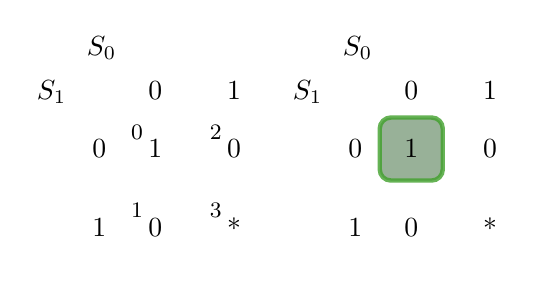
\begin{tikzpicture}
  \coordinate (a) at (0,0);
  \draw[draw=fg, thick] ($(a)+(-1,3)$) -- node[anchor = south west] {$S_0$} node[anchor = north east] {$S_1$} ++(1,-1);
  \draw[draw=fg, thick] (a) rectangle ++(2,2);
  \draw[draw=fg, thick] ($(a)+(0,1)$) -- ++(2,0);
  \draw[draw=fg, thick] ($(a)+(1,0)$) -- ++(0,2);
  \draw[] ($(a)+(0.5,2)$) node[rotate = 0, anchor = south] {0};
  \draw[] ($(a)+(1.5,2)$) node[rotate = 0, anchor = south] {1};
  \draw[] ($(a)+(0,0.5)$) node[rotate = 0, anchor = east]  {1};
  \draw[] ($(a)+(0,1.5)$) node[rotate = 0, anchor = east]  {0};

  \draw[] ($(a)+(0.5,1.5)$) node[anchor = south east, xshift = -1] {{\footnotesize 0}} node[rotate = 0, anchor = center] {1};
  \draw[] ($(a)+(0.5,0.5)$) node[anchor = south east, xshift = -1] {{\footnotesize 1}} node[rotate = 0, anchor = center] {0};
  \draw[] ($(a)+(1.5,1.5)$) node[anchor = south east, xshift = -1] {{\footnotesize 2}} node[rotate = 0, anchor = center] {0};
  \draw[] ($(a)+(1.5,0.5)$) node[anchor = south east, xshift = -1] {{\footnotesize 3}} node[rotate = 0, anchor = center] {*};

  \coordinate (b) at (3.25,0);
  \draw[draw=fg, thick] ($(b)+(-1,3)$) -- node[anchor = south west] {$S_0$} node[anchor = north east] {$S_1$} ++(1,-1);
  \draw[draw=fg, thick] (b) rectangle ++(2,2);
  \draw[draw=fg, thick] ($(b)+(0,1)$) -- ++(2,0);
  \draw[draw=fg, thick] ($(b)+(1,0)$) -- ++(0,2);
  \draw[] ($(b)+(0.5,2)$) node[rotate = 0, anchor = south] {0};
  \draw[] ($(b)+(1.5,2)$) node[rotate = 0, anchor = south] {1};
  \draw[] ($(b)+(0,0.5)$) node[rotate = 0, anchor = east]  {1};
  \draw[] ($(b)+(0,1.5)$) node[rotate = 0, anchor = east]  {0};

  \filldraw[fill=gr!50!bg, draw=gr, ultra thick, rounded corners, fill opacity = 0.5, draw opacity = 0.8] ($(b)+(0.1,1.1)$) rectangle ++(0.8,0.8);

  \draw[] ($(b)+(0.5,1.5)$) node[rotate = 0, anchor = center] {1};
  \draw[] ($(b)+(0.5,0.5)$) node[rotate = 0, anchor = center] {0};
  \draw[] ($(b)+(1.5,1.5)$) node[rotate = 0, anchor = center] {0};
  \draw[] ($(b)+(1.5,0.5)$) node[rotate = 0, anchor = center] {*};
\end{tikzpicture}
\end{document}
